\documentclass[a4paper, 11pt]{ctexart}
\usepackage[left=2.5cm, right=2.5cm, top=2.5cm, bottom=2.5cm]{geometry}
\usepackage{graphicx}
\usepackage{xcolor}
\usepackage{titlesec}
\usepackage{enumitem}
\usepackage{float}
\usepackage{booktabs}
\usepackage{siunitx}
\usepackage{subcaption}
\usepackage{url}

\setlength{\parindent}{0pt}
\setlength{\parskip}{0.5em}

\begin{document}

\begin{center}
\LARGE\textbf{算法计量与验证实验报告 - 第03章作业}\\[1em]
\large 姓名：\textbf{[Redacted]} \quad 学号：\textbf{[Redacted]}
\end{center}

\vspace{2em}

\textbf{运行环境说明}
\begin{itemize}[itemsep=0.2em, topsep=0.2em]
\item \textbf{操作系统：}macOS
\item \textbf{python版本：}3.12.7
\item \textbf{代码仓库：} \url{https://github.com/maidou07/dsa2026.git}
\end{itemize}

\section*{实验一：中缀表达式直接计算}

\subsection*{程序原理}

双栈法（操作数栈与运算符栈）从左至右扫描表达式。遇到操作数则压入操作数栈；遇到运算符则比较优先级，若栈顶运算符优先级不低于当前运算符，则弹出栈顶运算符并执行计算（从操作数栈弹出两个操作数），直至栈顶优先级更低或栈为空，再将当前运算符压入运算符栈。遇左括号压栈，遇右括号则弹栈计算直至匹配左括号。最终操作数栈顶即为结果。\\

实际实现封装了两个函数：\texttt{cal(op)} 和 \texttt{tokenize(s)}。前者执行每一次计算操作，封装提升代码简洁度；后者用于将不带空格的常规输入表达式拆分成计算函数可以处理的\texttt{tokens}。
\subsection*{测试用例与运行结果}

\begin{table}[H]
\centering
\begin{tabular}{clc}
\toprule
\textbf{编号} & \textbf{测试表达式} & \textbf{计算结果} \\
\midrule
用例1 & \texttt{2+3*4-4/2} & 12 \\
用例2 & \texttt{(2+3)*(4-1)} & 15 \\
用例3 & \texttt{((1+2)*(3+4))/3-8/4} & 5 \\
用例4 & \texttt{1+2*3-4/2+6*(7-8/2)+9/3*2} & 29 \\
\bottomrule
\end{tabular}
\caption{中缀表达式计算测试用例}
\end{table}

\subsection*{代码实现}

\begin{figure}[H]
\centering
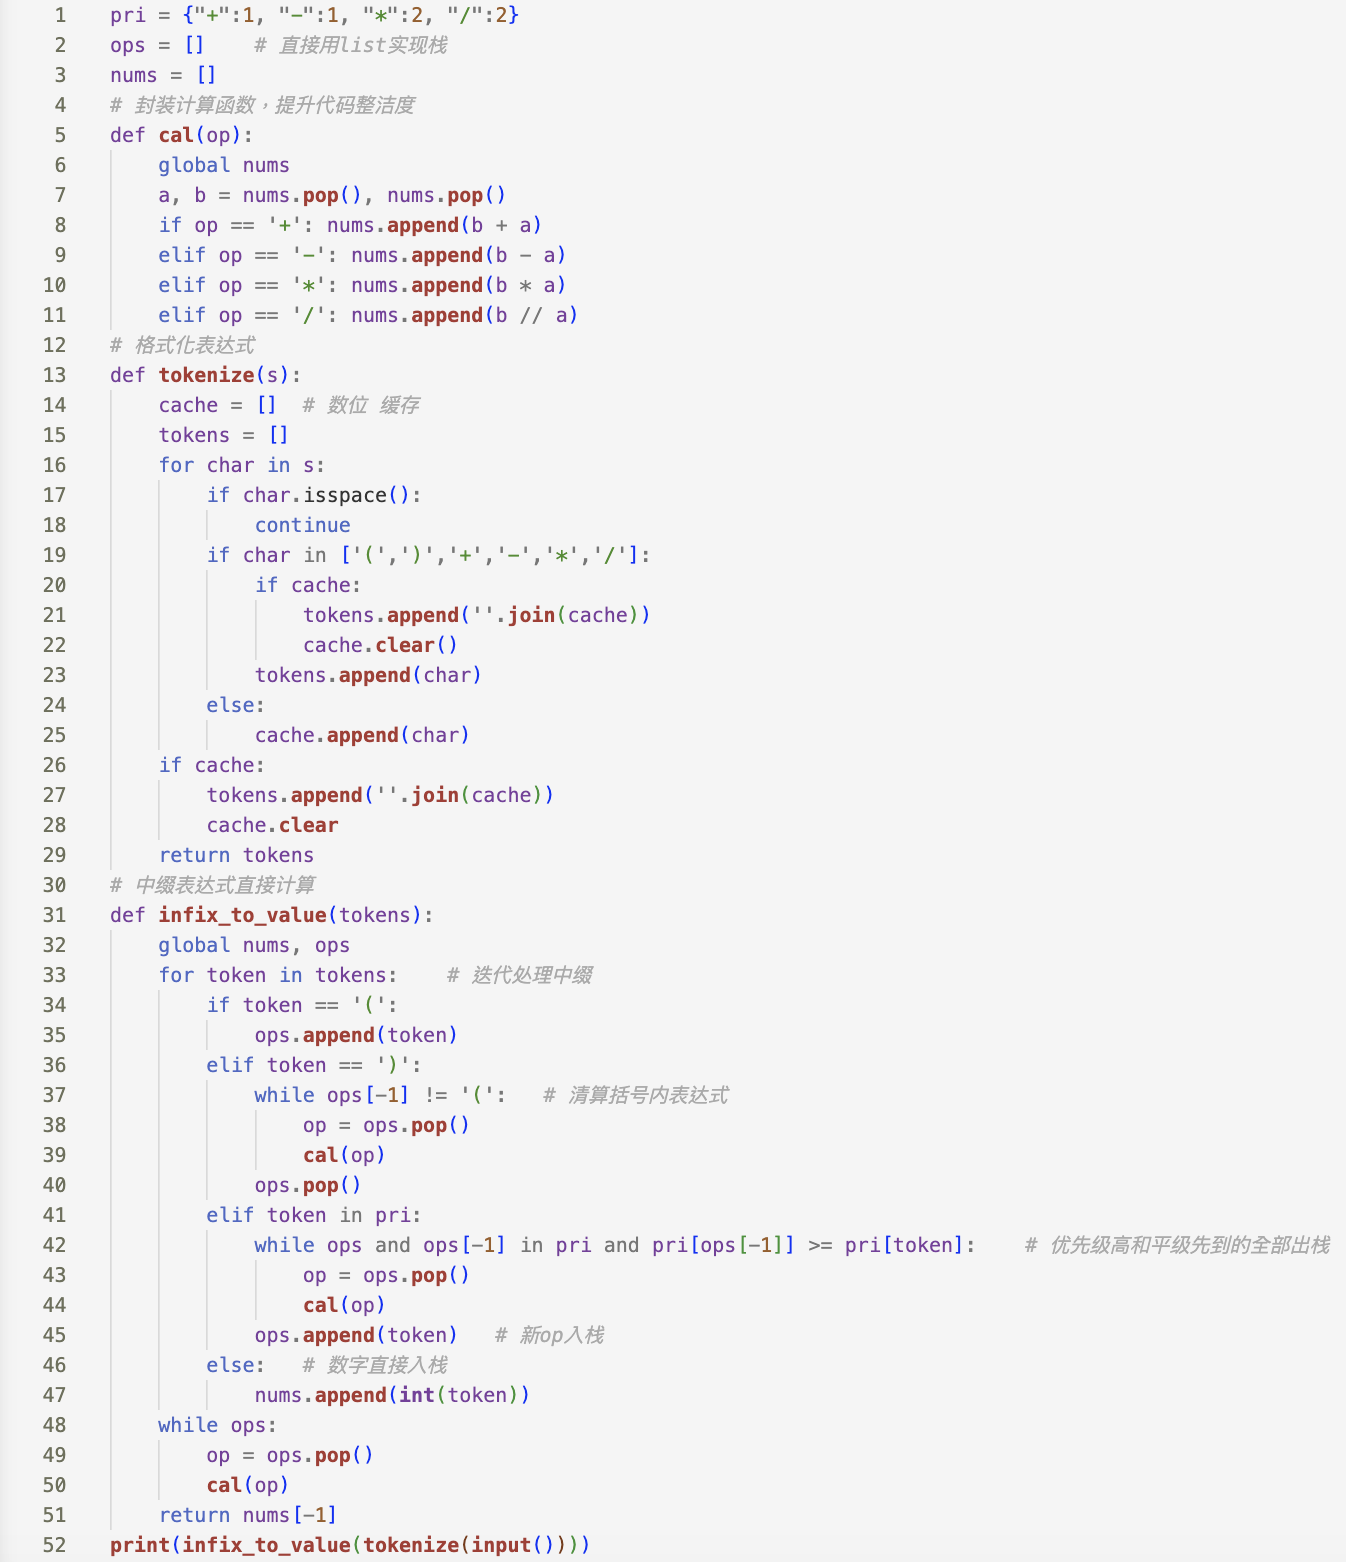
\includegraphics[width = 0.8 \textwidth]{../img/0301.png}
\end{figure}

\section*{实验二：队列性能对比实验}

\subsection*{程序原理}

List队列基于Python动态数组实现，底层为连续内存空间；入队时\texttt{append}在尾端追加元素，出队时\texttt{pop(0)}移除首元素。链表队列由游离节点类\texttt{ListNode}构成，通过头尾指针分别管理队首与队尾；入队创建新节点并链接至尾节点，出队只需移动头指针指向下一节点。

\subsection*{测试用例和运行结果}
分别测试三个数量级的队列，完整执行一套入队流程和全部出队流程，分别计时，得到以下的测试结果：
\begin{table}[H]
\centering
\begin{tabular}{ccS[table-format=3.5]S[table-format=4.5]}
\toprule
\textbf{数据规模} & \textbf{队列类型} & \textbf{入队耗时(ms)} & \textbf{出队耗时(ms)} \\
\midrule
1000 & LIST & 0.03187 & 0.12017 \\
     & LINKEDLIST & 0.17050 & 0.11879 \\
\midrule
10000 & LIST & 0.28838 & 4.90200 \\
      & LINKEDLIST & 1.59213 & 1.06058 \\
\midrule
100000 & LIST & 2.61971 & 575.11642 \\
       & LINKEDLIST & 14.84279 & 10.07296 \\
\bottomrule
\end{tabular}
\caption{队列性能对比测试结果}
\end{table}

\subsection*{实验分析}

\textbf{入队分析}：可以看到，在数据规模增长时，两者入队用时都成\textbf{线性增长}。这是因为两者的入队均为$O(1)$时间复杂度。List基于C数组实现，\texttt{append}操作在尾部追加，通过内置的均摊，可以保证每次插入都是常数开销。链表队列需每次创建一个新的\texttt{ListNode}对象，涉及内存分配与初始化，开销高于原生的C数组操作。因此\textbf{List入队略快于链表队列}。

\textbf{出队分析}：性能差异显著，完全出队的时间复杂度为$O(N^2)$与$O(1)$的差异。List的\texttt{pop(0)}移除首元素后，必须将后续$N-1$个元素整体前移一位以维持连续内存布局，时间复杂度$O(N)$。当连续执行$N$次出队时，总时间复杂度退化为$O(N^2)$，数据规模从10000增至100000时出队耗时从\SI{4.9}{\milli\second}飙升至\SI{575.1}{\milli\second}。链表队列出队仅修改头指针，不涉及数据移动，保持稳定的$O(1)$性能，出队耗时随规模\textbf{线性增长}（$100\times$数据仅约$100\times$耗时）。

\subsection*{代码实现}

\begin{figure}[H]
\centering
\begin{subfigure}[b]{0.8\textwidth}
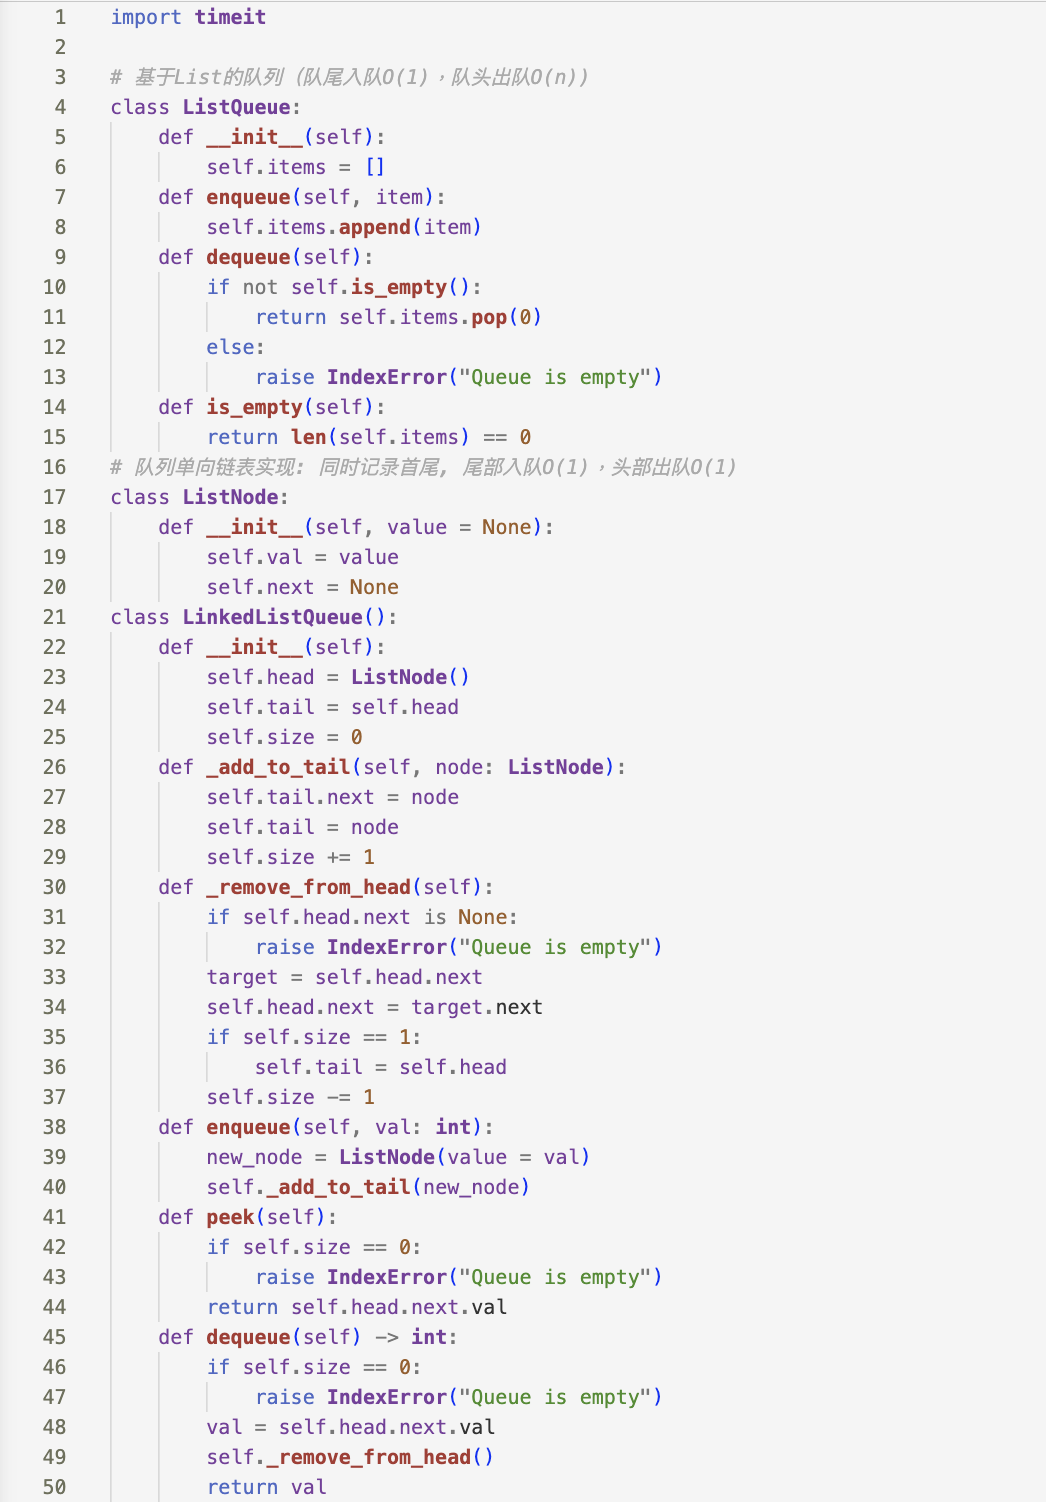
\includegraphics[width = \textwidth]{../img/0302_1.png}
\end{subfigure}
\begin{subfigure}[b]{0.8\textwidth}
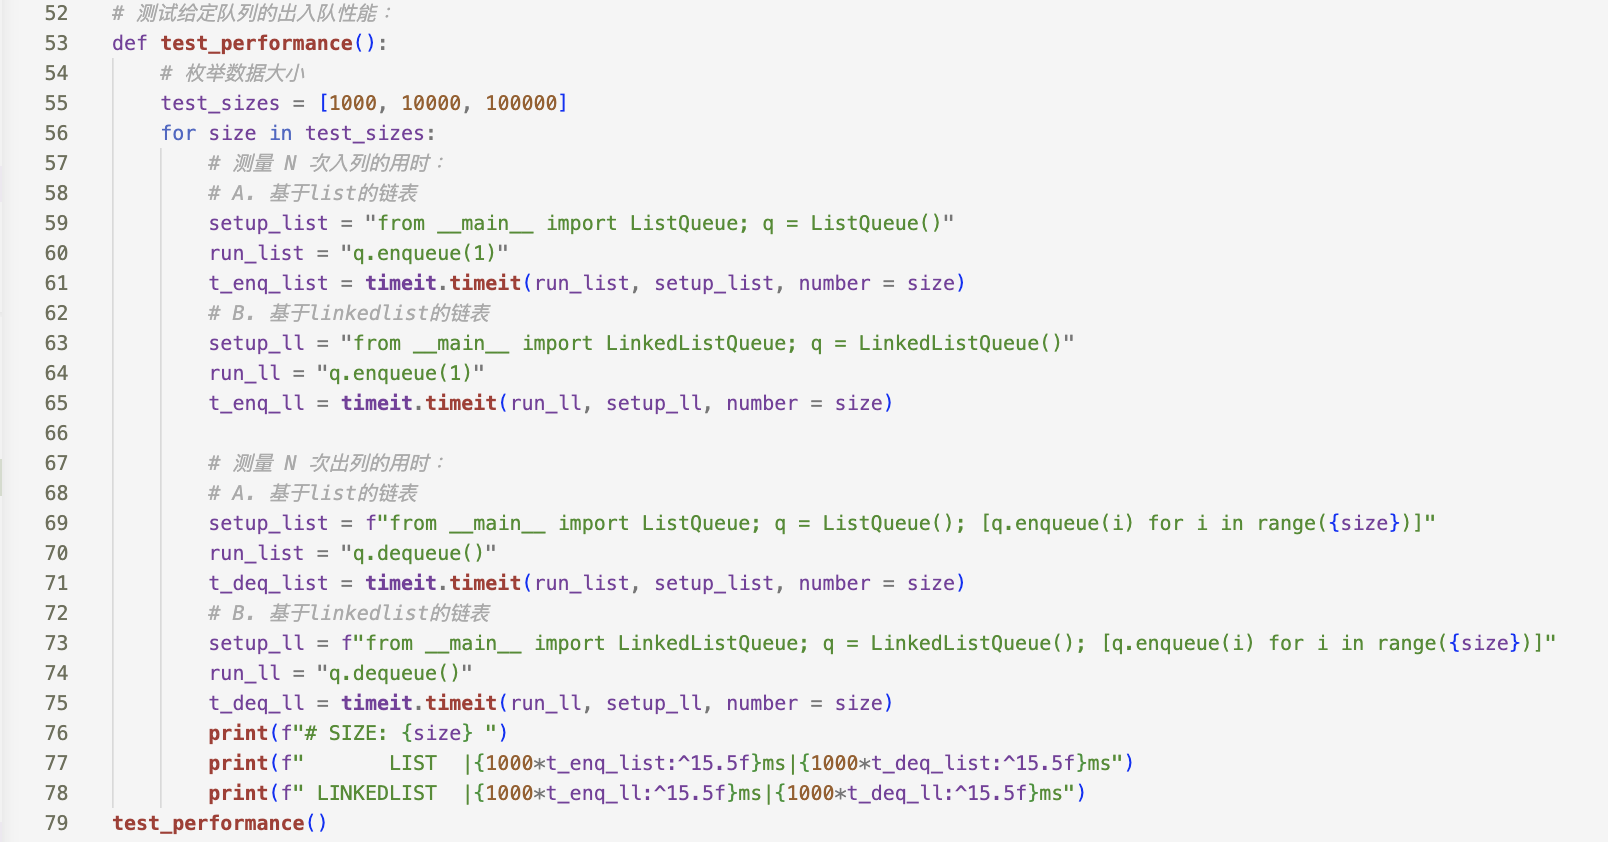
\includegraphics[width = \textwidth]{../img/0302_2.png}
\end{subfigure}
\end{figure}

\end{document}
